\documentclass{article}
\usepackage{graphicx}
\graphicspath{ {./images/} }
\usepackage{subcaption}
\usepackage[utf8]{inputenc}
\usepackage[margin=1in]{geometry}
\usepackage{hyperref}

\title{CMPS 287 - Final Project Report}
\author{Majd Al-Kawaas  \hspace*{5mm} \url{mma250@mail.aub.edu},\\  Melhem Rahmeh \hspace*{5mm} \url{mfr08@mail.aub.edu}, \\ Mohamed Louai Bouzaher \hspace*{5mm} \url{mlb03@mail.aub.edu},\\ Nathalie Nassar \hspace*{5mm} \url{nwn05@mail.aub.edu}

}
\date{May 2022}

\begin{document}

\maketitle

\section{Abstract}
Bot accounts have been a significant problem for social media websites especially Twitter and Reddit, most bots are harmful and they seek to create chaos or generate useless content on popular channels of social media communication. Our solution is a set of different machine learning models that performs Reddit bot detection on different sets of data about the users. We have chosen this approach to boost the accuracy of the results. \par

We have chosen comment/post level detection because account-level approaches require increased amounts of user data and there is a scarcity of [ADD HERE], whereas comments and posts can be analyzed using Natural Language Processing techniques.\par

The best model we propose is logistical regression, is it gave the highest accuracy for the 4 detection levels  we are approaching: \\
\begin{itemize}
\item User Posts Titles : $90.4\%$
\item Subreddits of User Posts: $92.3\%$
\item User Comments : $91.3\%$
\item Subreddits of User Comments : $90.5\%$

\end{itemize}

\section{Introduction}

Trolls and bots in social media are widespread, and it has been proven that they have unrecognized and significant effects on the users. The actions of a bot might affect our opinions, and thus the quality and accuracy of information we are getting. Moreover, some bots and trolls might be considered bad actors for having negative political, economic, and health effects. \par
Reddit, also known as "the front page of the internet,” is a social media platform for news aggregation and discussions. On Reddit, people are able to form communities around shared interests or sometimes shared dislikes. The power these communities wield is constantly increasing, and it was shown, a year ago, by the r/wallstreetbets subreddit; the participants of this subreddit were able to manipulate the stock market and drive the prices of GameStop stock to a significant number.  Furthermore,  a huge number of bots has been detected by the users and moderators on this specific subreddit. Another instance of bots interfering with the public opinion was annoucned in Reddit's Transparency report of 2017.  In this report have released more than 950 Russian bots accounts. These accounts were controlled by Russian organizations and most of their activities were focused on political communities on Reddit mostly relating to the 2016 US Election. In addition, some bots exist to downvote or upvote specific content or that of a specific user for marketing, or economic purposes. \par
While bot detection is being explored on other high profile platforms such as Twitter with deep learning, there is extremely limited work on bot detection applications on Reddit, and in the wake of the ever-changing political and economic scene, there is an increasing need for accurate methods of detecting bots on such platform given that they become a source of information for millions of users. Moreover, The nature of Reddit enables a very suitable environment for bots from all the existing social media platforms. The behavior of these bots, on Reddit, is turning some of the communities into unsafe and insecure online spaces that require termination.

\section{Related Work}
    As we have mentioned there is not much work on the Reddit bot detection issue but some parties are making some great efforts in this matter. Even Reddit never announced any in deepth details on their efforts or progress with this issue but some work on the matter has been done by Reddit community members.\par
    
     A group of graduate students at Stanford University worked on this problem for their thesis. They have applied deep learning to Reddit in an exploration of its viability in comment-level bot detection with a limited supervised dataset. They have performed a contextual analysis of the comments of these users using a variety of deep learning models and architectures (BERT and LSTM, RCNNs) they have achieved an AUC of 84.6\% using an RCNN architecture on their very minimal dataset.\par
     
     Medium project by Brandon Punturo, in this project the author dependent on the list of bots we are depending on. He built optimized random forest classifier and they final results and metrics were not promising.\par
     
     [ADD A PARAGRAPH ABOUT THE PAPER WE ARE USING OR NOT]
     
     Despite the fact that Reddit has significantly less labeled bot datasets than Twitter, the issue is gaining traction, and Reddit has escalated its attempts to combat it. The data of around 900 Russian troll accounts that submitted over 7000 total comments was revealed in Reddit's 2017 transparency report, producing an extremely limited but workable supervised dataset. This list or Russian bots was started by a professor at Boston University and then Reddit took over the process \par
     
     
    %  The only similar work on comment level identification currently available is a Medium project by Brandon Punturo, \par

    
\section{Dataset}
Our process of acquiring the data follows these steps:
    \begin{enumerate}
        \item Identify verified lists of bot accounts (Reddit 2017 transparency Report, autowikibot, botwatch)
        \item Scrap the username of the account from their respective web pages.
        \item Identify a list of normal users that were active during the same time the bot accounts were active.
        \item Retrieve the accounts posts, and comments using the Reddit official API, and the PushShift API (Unofficial API).
        \item Store the data in a MongoDB server given that a user has multiple comments and posts and storing this data as CSV means storing the parts of the data multiple times.\\
        That's the database diagram, and you can find the dataset explanation below.\\ \\
            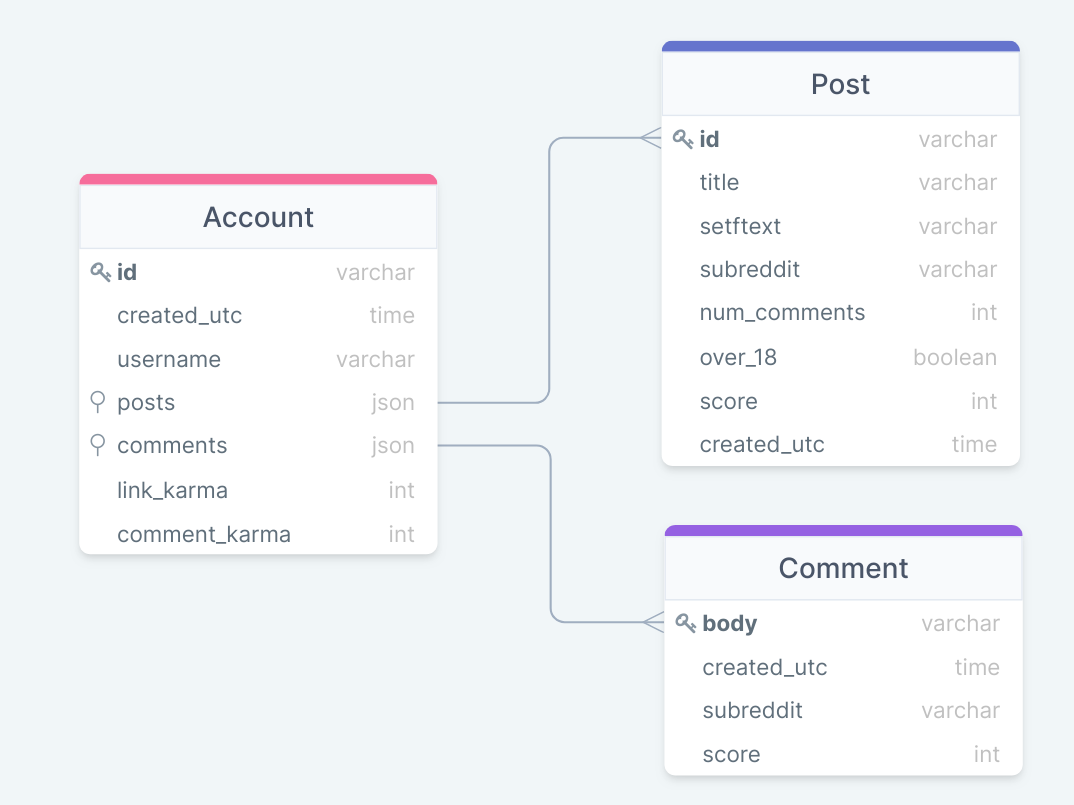
\includegraphics[width=10cm, height=8cm]{db}\\
        \item Retrieve the required data depending on the model i.e training the comments body model we retrieve the comments and the label of all the users in our data. \\ \\
    \end{enumerate}
The dataset consist of three main parts and each part has of the following features:
    \begin{enumerate}
        \item User Data
            \begin{enumerate}
                \item username
                \item cakeday: (user account creation date)
                \item comment karma: value of the sum of a given user's upvotes and downvotes.
                \item post karma.
                \item is bot: A boolean value added by us during the process of retrieval chosen depending on the source of the username (from list of bots or not).
            \end{enumerate}
        \item Post Data
            \begin{enumerate}
                \item comment body
                \item creation date: a timestamp of date and time.
                \item subreddit: the subreddit at with comment was posted.
            \end{enumerate}
        \item Comment Data
            \begin{enumerate}
                \item post title
                \item post body
                \item number of comments
                \item creation date: a timestamp of date and time.
                \item subreddit: the subreddit at which the post was posted.
            \end{enumerate}
    \end{enumerate}

    
\section{Model}
    Given that we have different types of data (dates, comment/post title) we have four different models each handling a different form of data. This also contributed to boosting the accuracy given that [ADD HERE].\\
    For each portion of the
    We have a the following models
    \begin{enumerate}
        \item comment subreddit model
        \item comment body model
        \item Post title model
        \item Post subreddit model
    \end{enumerate}
    
For each one of the mentioned models, we experimented with different combinations of the following models: SVM , Logistical Regression, Neural Networks , KNN and Naive Bayes. 
        \begin{itemize}
        \item \textbf{SVM}:  The SVM model was proposed by Cortes and Vapnik. It is a supervised learning model mostly used for classification and regression problems. The SVM aims at calculating the weights w and bias b such that the hyperplane found perfectly separates the data while maximizing the margin.
    
    For an efficient non-linear transformation, we used kernels.
    
    The first kernel used was linear and the second was polynomial.
        \item \textbf{Logistical Regression} :     Logistic regression is a statistical model used for binary classification, and it can be generalized to multiclass classification. \\
Logistic regression uses the Sigmoid Function, that is $\frac{1}{1+e^{-x}}$\\ \\ It outputs a value between 0 and 1, that's the probability if the positive label class. Here, it's the $isBot$ label, and if it's greater than 0.5, the $isBot$ will be equal $True$, else the $isBot$ will be equal $False$.  \\ \\
Logistic Regression try to minimize the "cross-entropy error", that is:\\ $\frac{1}{N} \sum_{n=1}^{N} ln(1 + e^ {-y_{n}w^Tx_n}) = 1$\\ \\
It is an extensively employed algorithm for classification in industry because of it's simplicity and good results. \\

        \item \textbf{Neural Networks}     Neural network is based on contextual long short-term memory architecture that exploits both content and metadata to detect bots at the post level: the pre-processed data was fed as  input to the network in order to see whether it consists of a bot or genuine user. 
    
    After the training using the ReLU activation function for the deep layers and Sigmoid activation function for the output layer knowing it consists of a binary classification.
    
    After training for 100 epochs, the accuracy on the test dataset was 0.89.

        \item \textbf{KNN}: Briefly, K-NN algorithm assumes the similarity between the new case/data and available cases and put the new case into the category that is most similar to the available categories.

        \item \textbf{Naive Bayes}:     Naive Bayes classifiers are a collection of classification algorithms based on Bayes’ Theorem.
\\ \\ \\ \\ \\
        \end{itemize} 
        

    \subsection{Comment Subreddit}
    The comment subreddit is the subreddit at which the comment was posted. \\
    During the classification of  the subreddit model, we used three models in order to evaluate their efficiency in correctly predicting bots from normal users. For that, we used: Support Vectors Machine(SVM), Logistic Regression, and Neural Networks.
    For logistical Regression and SVM, we performed hyperparameter tuning using grid search, and random search for neural networks.
 
        \begin{center}
    \begin{tabular}{|c || c| c|} 
     \hline
     Model & Accuracy  & F1 Score  \\ [0.5ex] 
     \hline\hline
     SVM Linear & 0.86  &0.83 \\ 
     \hline
     SVM Polynomial & 0.86 &0.84 \\
     \hline
     Logistical Regression & 0.87 & 0.84  \\ 
     \hline
     Neural Networks & 0.84  & 0.82\\
     \hline

    \end{tabular}
    \end{center}

    \subsection{Comment Body}
    During the classification of  the subreddit model, we used three models in order to evaluate their efficiency in correctly predicting bots from normal users. For that, we used: Support Vectors Machine(SVM), Logistic Regression, and Neural Networks.
    For logistical Regression and SVM, we performed hyperparameter tuning using grid search, and random search for neural networks.
        \begin{center}
    \begin{tabular}{|c || c| c|} 
     \hline
     Model & Accuracy  & F1 Score  \\ [0.5ex] 
     \hline\hline
     SVM Linear & 0.90  & 0.88 \\ 
     \hline
     SVM Polynomial & 0.91 &0.90 \\
     \hline
     Logistical Regression & 0.91 & 0.91  \\ 
     \hline
     Neural Networks & 0.90  & 0.90\\
     \hline

    \end{tabular}
    \end{center}


    \subsection{Post Title}
    The post title is the text of the post title. \\
    We did not consider the posts bodies as it has no limit, and can include videos, images, tables, index tables...\\
    During the classification of  the Post Title model, we used four models in order to evaluate their efficiency in correctly predicting bots from normal users. For that, we used:         Support Vector Machines, Logistical Regression , Naive Bayes and KNN.
    For logistical Regression, SVM, KNN, we performed hyperparameter tuning using grid search, random search for neural networks, and no hyperparameter tuning for Naive Bayes, as there are parameters to tune.

        \begin{center}
    \begin{tabular}{|c || c| c|} 
     \hline
     Model & Accuracy  & F1 Score  \\ [0.5ex] 
     \hline\hline
     SVM Linear & 0.89  & 0.89 \\ 
     \hline
     KNN & 0.87 & 0.84 \\
     \hline
     Naive Bayes & 0.61 &0.66 \\
     \hline
     Logistical Regression & 0.91 & 0.89  \\ 
     \hline
    \end{tabular}
    \end{center}
    
    \subsection{Post subreddit}  
    
        The comment subreddit is the subreddit at which the post was posted. \\
    During the classification of  the subreddit model, we used three models in order to evaluate their efficiency in correctly predicting bots from normal users. For that, we used: Support Vectors Machine(SVM), Logistic Regression, and Neural Networks.
For logistical Regression and SVM, we performed hyperparameter tuning using grid search, random search for neural networks.

        \begin{center}
    \begin{tabular}{|c || c| c|} 
     \hline
     Model & Accuracy  & F1 Score  \\ [0.5ex] 
     \hline\hline
     SVM Linear & 0.91  & 0.90 \\ 
     \hline
     SVM Polynomial & 0.89 &0.89 \\
     \hline
     Logistical Regression & 0.90 & 0.90  \\ 
     \hline
     Neural Networks & 0.90  & 0.89\\
     \hline

    \end{tabular}
    \end{center}        
\section{Results}
    
    \subsection{Learning curves}
    
    \begin{figure}
  \begin{subfigure}[t]{.5\textwidth}
    \centering
    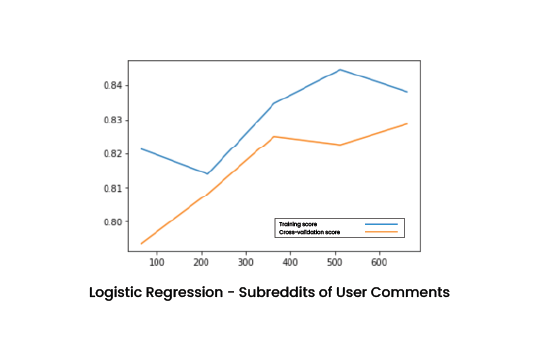
\includegraphics[width=\linewidth]{1}
  \end{subfigure}
  \hfill
  \begin{subfigure}[t]{.5\textwidth}
    \centering
    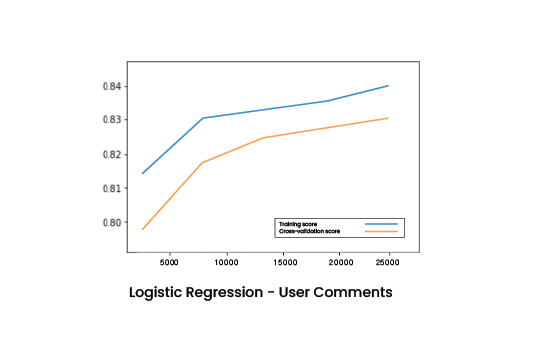
\includegraphics[width=\linewidth]{2}
  \end{subfigure}

  \medskip

  \begin{subfigure}[t]{.5\textwidth}
    \centering
    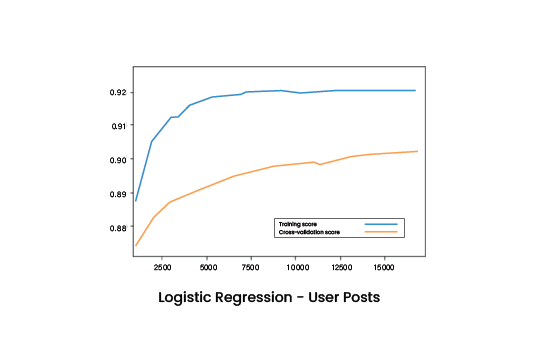
\includegraphics[width=\linewidth]{3}
  \end{subfigure}
  \hfill
  \begin{subfigure}[t]{.5\textwidth}
    \centering
    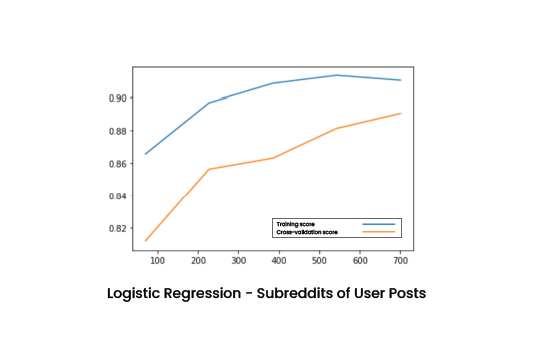
\includegraphics[width=\linewidth]{4}
  \end{subfigure}
\end{figure}
        
    \subsection{Classification Reports / Confusion matrices}
The best model for all 4 detection level is logistical regression. \\ \\
    \begin{tabular}{ |p{3.5cm}||p{3cm}|p{3cm}| p{3cm}|p{3cm}|  }
\hline
 Model / Metric & F1 Score & Accuracy& Precision & Support \\
 \hline
 Comment Subreddit   & 0.90    &0.91 & 0.90& 553\\
  Comment Body   & 0.91    & 0.91 & 0.92 & 20238\\
  Post Title & 0.89    &0.90 & 0.90 & 24917 \\
  Post Subreddit  & 0.92    &0.92 & 0.93 & 585\\
 \hline
\end{tabular}

 
 \section{Conclusion}
 Detecting bots by analyzing their behavior is a difficult task, since they can behave approximately like any other user. However, inspecting the language they use to post and comment and the pattern they follow to do so, helps us understand and detect them with high accuracy.

\end{document}